\frame{
  \begin{block}{Log-replay examples}
    Trace log $(A, 1s), (B, 2s), (D, 8s)$ 
  \end{block}
  \begin{center}
    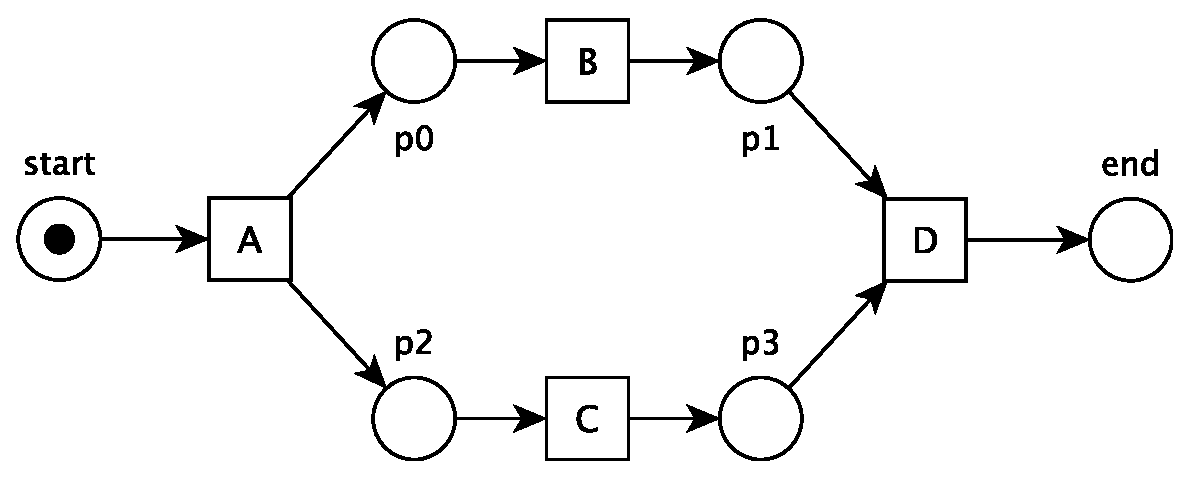
\includegraphics[scale=0.30]{./fig/LogReplay1a}
  \end{center}
  \begin {block}{Measures}
    \begin{tabular}{cc}
    \end{tabular}
  \end{block}
}
\frame{
  \begin{block}{Log-replay examples}
    Trace log $\alert{(A, 1s)}, (B, 2s), (D, 8s)$ 
  \end{block}
  \begin{center}
    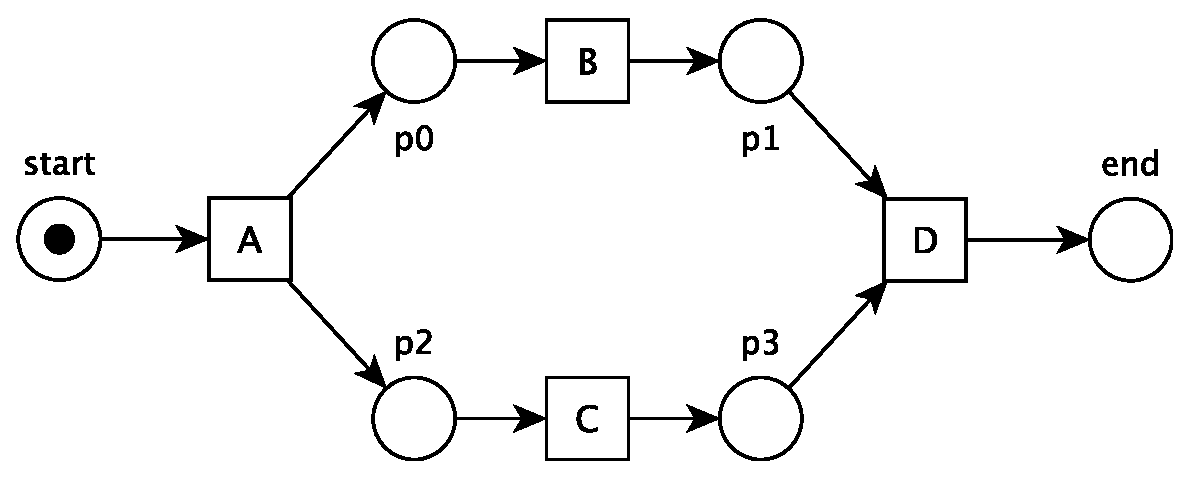
\includegraphics[scale=0.30]{./fig/LogReplay1a}
  \end{center}
  \begin {block}{Measures}
    \begin{tabular}{cc}
    \end{tabular}
  \end{block}
}
\frame{
  \begin{block}{Log-replay examples}
    Trace log $\alert{(A, 1s)}, (B, 2s), (D, 8s)$ 
  \end{block}
  \begin{center}
    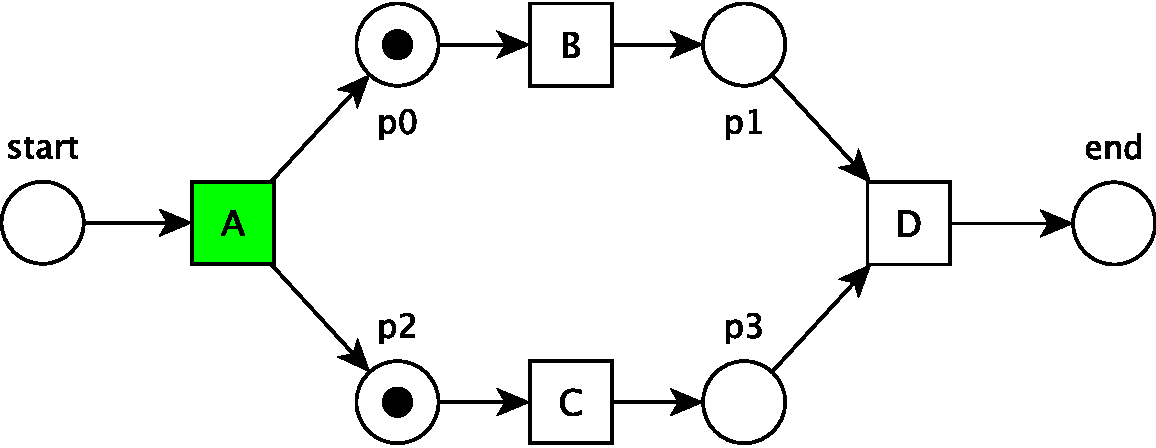
\includegraphics[scale=0.30]{./fig/LogReplay1b}
  \end{center}
  \begin {block}{Measures}
    \begin{tabular}{ccc}
                  & p0 & p2 \\
       $\TSync$   & 0  & 0  \\
    \end{tabular}
  \end{block}
}
\frame{
  \begin{block}{Log-replay examples}
    Trace log $(A, 1s), \alert{(B, 2s)}, (D, 8s)$ 
  \end{block}
  \begin{center}
    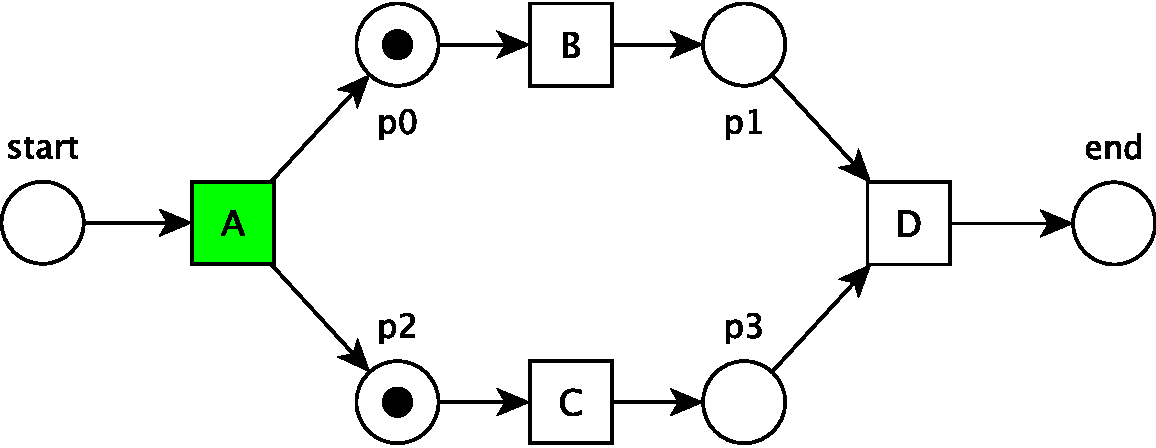
\includegraphics[scale=0.30]{./fig/LogReplay1b}
  \end{center}
  \begin {block}{Measures}
    \begin{tabular}{ccc}
                  & p0 & p2 \\
       $\TSync$   & 0  & 0  \\
    \end{tabular}
  \end{block}
}
\frame{
  \begin{block}{Log-replay examples}
    Trace log $(A, 1s), \alert{(B, 2s)}, (D, 8s)$ 
  \end{block}
  \begin{center}
    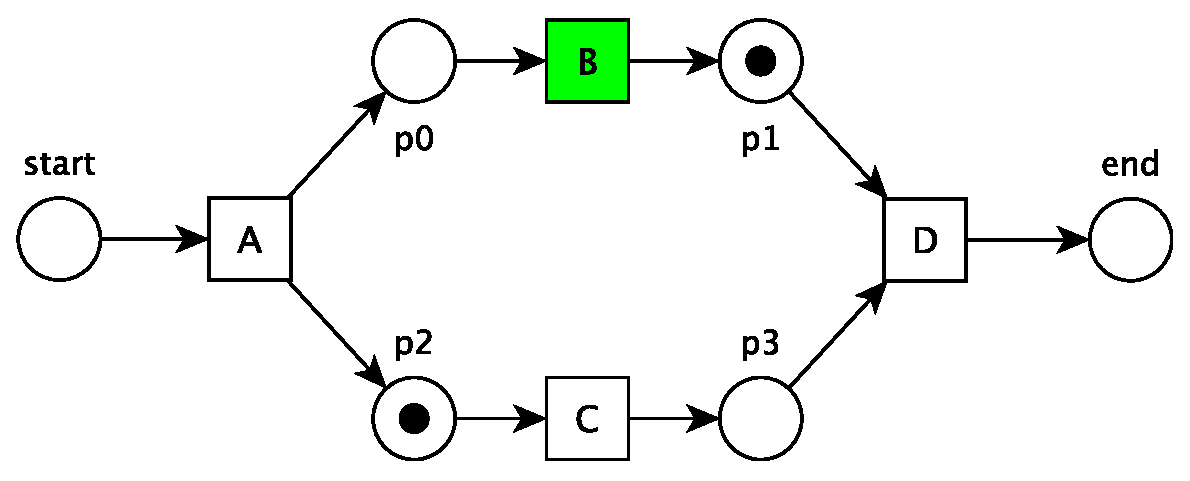
\includegraphics[scale=0.30]{./fig/LogReplay1c}
  \end{center}
  \begin {block}{Measures}
    \begin{tabular}{ccc}
                  & p0 & p2 \\
       $\TSync$   & 0  & 0  \\
       $\TTot$    & 1  &    \\
    \end{tabular}
  \end{block}
}
\frame{
  \begin{block}{Log-replay examples}
    Trace log $(A, 1s), (B, 2s), \alert{(D, 8s)}$ 
  \end{block}
  \begin{center}
    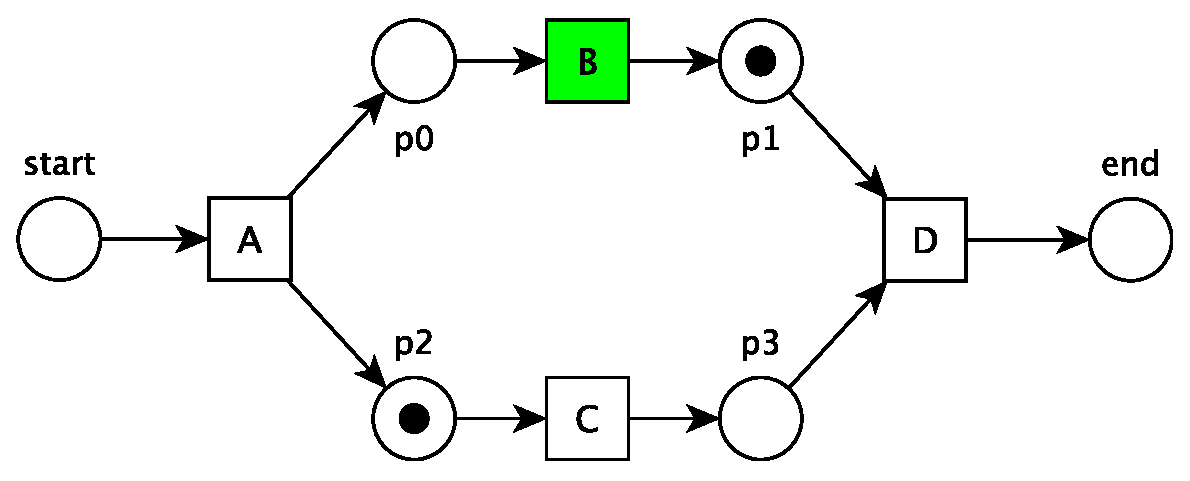
\includegraphics[scale=0.30]{./fig/LogReplay1c}
  \end{center}
  \begin {block}{Measures}
    \begin{tabular}{ccc}
                  & p0 & p2 \\
       $\TSync$   & 0  & 0  \\
       $\TTot$    & 1  &    \\
    \end{tabular}
  \end{block}
}

\frame{
  \begin{block}{Log-replay examples}
    Trace log $(A, 1s), (B, 2s), \alert{(D, 8s)}$ 
  \end{block}
  \begin{center}
    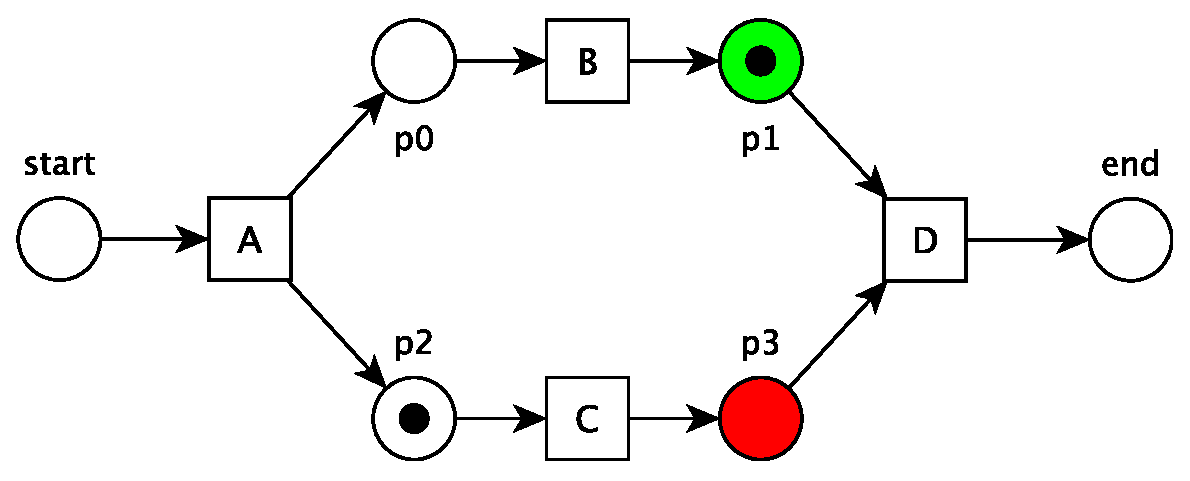
\includegraphics[scale=0.30]{./fig/LogReplay2d}
  \end{center}
  \begin {block}{Measures}
    \begin{tabular}{ccc}
                  & p0 & p2 \\
       $\TSync$   & 0  & 0  \\
       $\TTot$    & 1  &    \\
    \end{tabular}
  \end{block}
}
\frame{
  \begin{block}{Log-replay examples}
    Trace log $(A, 1s), (B, 2s), \alert{(D, 8s)}$ 
  \end{block}
  \begin{center}
    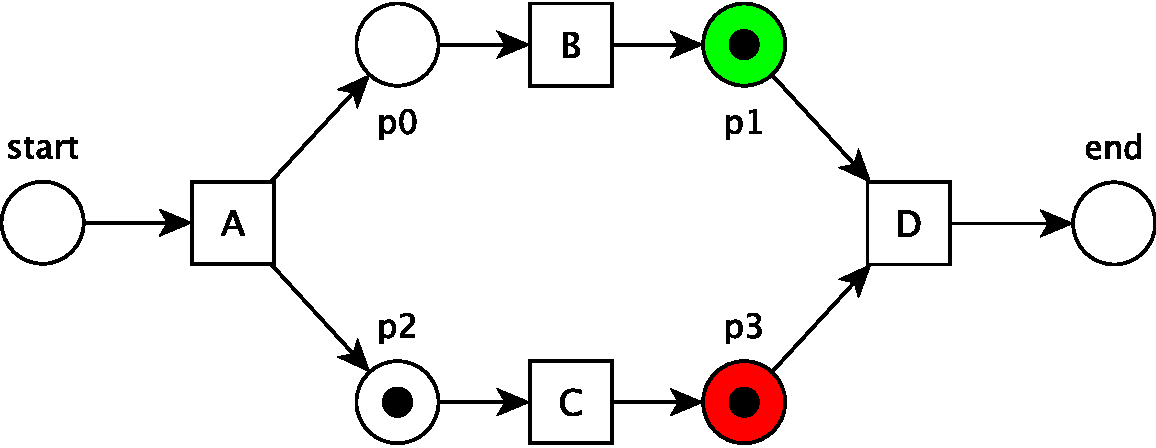
\includegraphics[scale=0.30]{./fig/LogReplay2f}
  \end{center}
  \begin {block}{Measures}
    \begin{tabular}{ccc}
                  & p0 & p2 \\
       $\TSync$   & 0  & 0  \\
       $\TTot$    & 1  &    \\
    \end{tabular}
    \begin{tabular}{ccc}
                  & p3 \\
       $Missing$  & 1  \\
    \end{tabular}
  \end{block}
}
\frame{
  \begin{block}{Log-replay examples}
    Trace log $(A, 1s), (B, 2s), \alert{(D, 8s)}$ 
  \end{block}
  \begin{center}
    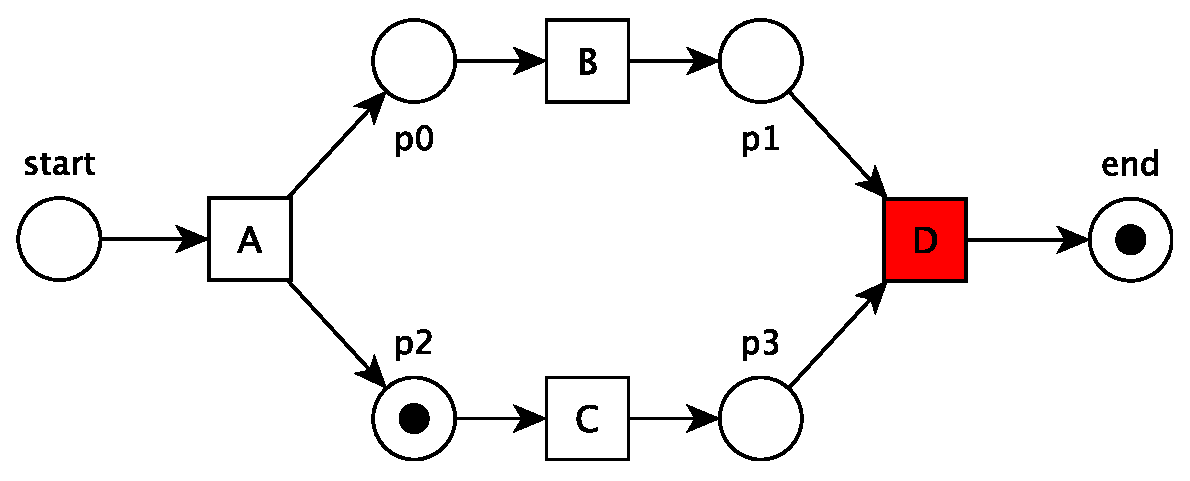
\includegraphics[scale=0.30]{./fig/LogReplay2g}
  \end{center}
  \begin {block}{Measures}
    \begin{tabular}{ccc}
                  & p0 & p2 \\
       $\TSync$   & 0  & 0  \\
       $\TTot$    & 1  &    \\
    \end{tabular}
    \begin{tabular}{ccc}
                  & p3 \\
       $Missing$  & 1  \\
    \end{tabular}
  \end{block}
}
\frame{
  \begin{block}{Log-replay examples}
    Trace log $(A, 1s), (B, 2s), \alert{(D, 8s)}$ 
  \end{block}
  \begin{center}
    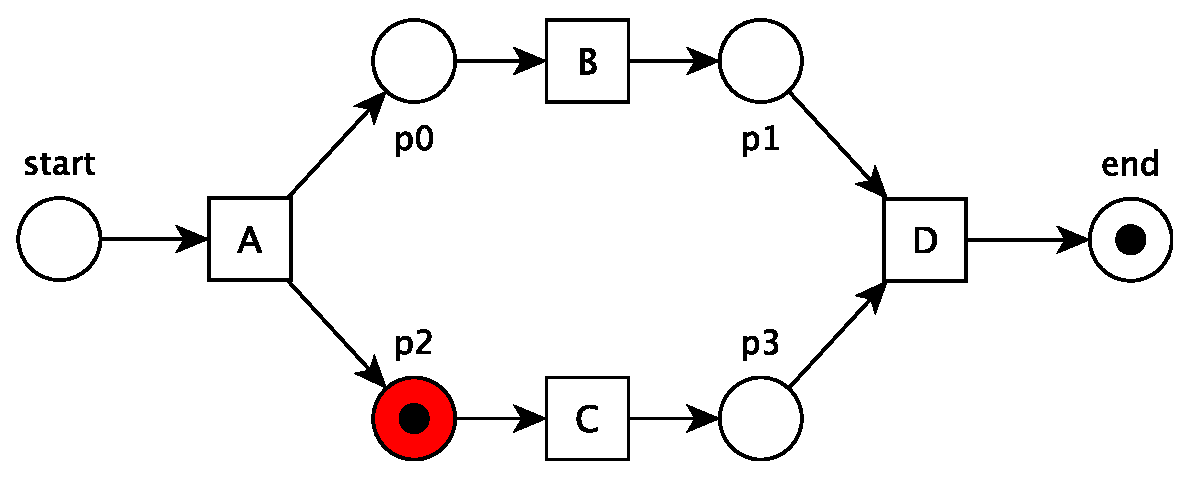
\includegraphics[scale=0.30]{./fig/LogReplay2h}
  \end{center}
  \begin {block}{Measures}
    \begin{tabular}{ccc}
                  & p0 & p2 \\
       $\TSync$   & 0  & 0  \\
       $\TTot$    & 1  &    \\
    \end{tabular}
    \begin{tabular}{ccc}
                   & p3 & p2 \\
       $Missing$   & 1  & 0  \\
       $Remaining$ & 0  & 1   \\
    \end{tabular}
  \end{block}
}


%%% Local Variables: 
%%% mode: latex
%%% TeX-master: "main"
%%% End: 
